
\section{Introduction}
At high frequencies and amplitudes, the propagation of sound waves is described by quasilinear wave equations. In complex tissue-like media, additionally, nonlocal attenuation effects become apparent. In practice, the involved dissipation parameter is relatively small and becomes negligible in inviscid media. It is thus important to establish conditions under which numerical simulation methods remain stable and accurate across different attenuation scales. Simulation of such nonlinear and nonlocal models is especially relevant for advancing medical applications of ultrasound waves in imaging~\cite{szabo2004diagnostic} and the treatment of solid tumors~\cite{kennedy2005high}. With this motivation in mind, we investigate  finite element discretizations  of the following class of nonlinear wave equations:
\begin{equation} \label{model_eq}
	\begin{aligned}
	(\mathfrak{a}(u^\eps) \ut^\eps)_t-c^2\Delta u^\eps-\varepsilon \Delta \frakK*\ut^\eps=f,
	\end{aligned}
\end{equation}
that are robust with respect to the parameter $\eps<<1$ , where
\[
\aaa(u^\eps)=1+ku^\eps, \quad k \in \R,
\]
and $*$ denotes the Laplace convolution in time. Originally derived by Westervelt in~\cite{westervelt1963parametric} for inviscid media with $\eps=0$, in thermoviscous media it involves $\frakK=\delta_0$ (the Dirac delta distribution) and thus the strong damping $-\eps \Delta \ut^\eps$. The damping parameter is then known as the sound diffusivity~\cite{lighthill1956viscosity} as it contributes to the parabolic-like character of the model. The vanishing limit is thus singular as there is a change from parabolic-like to hyperbolic evolution.  In complex media, $\frakK$ is weakly singular. It may be given by the Abel fractional kernel:
\begin{equation} \label{Abel_krenel}
	\frakK= \frac{1}{\Gamma(1-\alpha)}t^{-\alpha} \quad \alpha \in (0,1),
\end{equation}
where $\Gamma(\cdot)$ is the Gamma function. In that case the resulting dissipation term is $-\eps \Delta \textup{D}_t^\alpha u$, where $\textup{D}_t^\alpha$ is the Caputo--Djrbashian derivative of order $\alpha$. Mittag-Leffler-type kernels are also of interest; we refer to~\cite{kaltenbacher2022limiting} and Section~\ref{Sec:TheoreticalPreliminaries} for details. We unify these different cases of interest into one model in \eqref{model_eq} by imposing general non-restrictive regularity and sign conditions on $\frakK$; see Section~\ref{Sec:TheoreticalPreliminaries}. \\
\indent \indent The goal of this work is twofold. First, we wish to determine sufficient conditions for a uniform conforming finite element discretization of \eqref{model_eq} with respect to $\varepsilon$. In other words, we wish to arrive at stability and \emph{a priori} error estimates for the corresponding semi-discrete solution where the involved constant does not blow up as $\varepsilon \rightarrow 0$.  Secondly, we aim to establish whether the vanishing dissipation asymptotics is preserved on the discrete level. These properties are visualized in the diagram in Figure~\ref{Fig:Diagram}. The present work fits into the wider class of studies on asymptotic-preserving numerical methods; see, e.g.,~\cite{jin2022asymptotic, degond2017asymptotic, feireisl2018asymptotic}, and the references provided therein. Remarkably, such methods permit discretizing the preturbed and limit problems with the same discretization parameters. 
\begin{figure}[h]
	\adjustbox{scale=1.1,center}{
		\begin{tikzcd}[row sep=huge, column sep = huge]
		\ref{Ph_nl} \arrow[r, dashed, "h \rightarrow 0"] \arrow[d, dashed, "\eps \rightarrow 0"]
		& \ref{P_nl}  \arrow[d, "\eps \rightarrow 0"] \\
		\ref{Ph_nl_zero} \arrow[r                                                                                                                                                                                                                                                                                                                                                                                                                                                                                                                                                                                                                                          , "h \rightarrow 0"]
		&  \ref{P_nl_zero}
		\end{tikzcd}
	}
	\caption{Asymptotic Preserving diagram: This work establishes the connection between \ref{Ph_nl} and \ref{P_nl} as $h \rightarrow$ 0, uniformly in $\eps$, as well as between \ref{Ph_nl} and \ref{Ph_nl_zero} as $\eps \rightarrow 0$.} \label{Fig:Diagram}
\end{figure} 
\subsection*{Main contributions} Our main results provide sufficient conditions under which the following convergence rates hold:
		\begin{equation} \label{eps_conv_1}
\begin{aligned}
\|u^\eps-\uh^\eps\|_{W^{2,\infty}(0,T; \Ltwo)}+h\|\nabla(u^\eps-\uh^\eps)\|_{W^{1,\infty}(0,T; \Ltwo)} \leq C h^r
\end{aligned}
\end{equation}
with $d/2<r \leq p+1$ and $p$ being the polynomial degree of the finite element space, and
		\begin{equation} \label{eps_conv_2}
	\begin{aligned}
		\|\uh^\eps-\uh^0\|_{L^\infty(0,T; \Ltwo)} \leq C {\eps},
	\end{aligned}
\end{equation}
where the involved constants do not depend on $h$ or $\eps$. To the best of our knowledge, this is the first such result in the context of nonlinear and nonlocal acoustic equations. In terms of the closely related works, we point out the non-uniform finite element analysis of the local Westervelt equation (with $\frakK=\delta_0$ and $\eps>0$)  in \cite{nikolic2019priori}. Finite element analysis of the inviscid problem ($\frakK=\delta_0$ and $\eps=0$) follows as a special case of the results in~\cite{hochbruck2022error, dorich1173strong}. Uniform-in-$\eps$ analysis of a mixed finite element approximation of the local Westervelt equation in the so-called potential form (with $\frakK=\delta_0$ and $\aaa=1+k \ut^\eps$) is available in \cite{Meliani2022}. Analysis of a time-discretization of \eqref{model_eq} with fractional-type damping has been performed in~\cite{baker2022numerical}. \\
\indent The core of the analysis arguments of our approach lies in devising semi-discrete energy functionals for which the approximate solution $\uh^\eps$ is uniformly bounded in $\eps$. The uniform energy analysis is first carried out on a linearized problem with $\aaa=\aaa(x,t) \geq \ulal >0$ and then transferred to a nonlinear one through a fixed-point argument in the spirit of, e.g.,~\cite{makridakis1993finite, ortner2007discontinuous, nikolic2019priori}.  For this fixed-point argument to work, it is essential that a uniform bound is established  on $\uhtt^\eps$ in a suitable norm. This leads to having to consider also the time-differentiated problem and involve higher-order energy functionals compared to the non-uniform finite-element analysis; cf.~\cite{nikolic2019priori}. Note that the energy maneuvers are considerably restricted by ({\bf 1})  ensuring the non-degeneracy of the leading factor $1+k \uh^\eps \geq \ulal>0$, and ({\bf 2}) the positivity properties one can expect from the (in general, fractional-type)  kernels. Thus there is a delicate interplay of nonlinearity, nonlocality, and potential degeneracy of the problem to consider.
\subsection*{Organization of the paper} We organize the rest of the exposition as follows. In Section~\ref{Sec:TheoreticalPreliminaries}, we discuss the assumptions on the kernel and provide details on the semi-discretization. Section~\ref{Sec:LinearAnalysis} contains the uniform stability and \emph{a priori} error analysis of the linearized problem. Section~\ref{Sec:NonlinearAnalysis} relates these results to the nonlinear problem using Schauder's fixed-point theorem, under suitable smallness conditions on the discretization parameter and the exact solution, independently of $\eps$. In Section~\ref{Sec:EpsLimit}, we prove \eqref{eps_conv_2} and also illustrate the theory with a numerical example. The main theoretical results are contained in Theorems~\ref{Thm:WellpNl} and~\ref{Thm:epsConv_lower}. 
\section{Problem setting} \label{Sec:TheoreticalPreliminaries}
Let $\Omega \subset \mathbb{R}^d$ be an interval ($d=1$), or a convex polygonal ($d=2$) or polyhedral ($d=3$) domain. Given final time $T>0$, we consider the following initial boundary-value problem for the (in general) nonlocal Westervelt equation: 
\begin{equation} \label{P_nl} \tag{\ensuremath{{\bf {P}}^{\varepsilon}}}
\left\{ \begin{aligned}
&(((1+k u^\eps)\ut^\eps)_t, \phi)_{L^2}+(c^2\nabla u^\eps+\varepsilon \nabla \frakK*\ut^\eps, \nabla \phi)_{L^2}= (f, \phi)_{L^2}, \\[2mm]
&\text{for all } \phi\in H_0^1(\Omega) \text{ a.e.\ in time, with}  \\[2mm]
&(u^\eps, \ut^\eps)\vert_{t=0}=	(u_{0}, u_{1}),
\end{aligned} \right.
\end{equation}
where $(\cdot, \cdot)_{L^2}$ denotes the scalar product on $L^2(\Omega)$. The limiting problem is given by
\begin{equation} \label{P_nl_zero} \tag{\ensuremath{{\bf {P}}^{0}}}
\left\{ \begin{aligned}
&(((1+k u^0)\ut^0)_t, \phi)_{L^2}+(c^2\nabla u^0, \nabla \phi)_{L^2}= (f, \phi)_{L^2}, \\[2mm]
&\text{for all } \phi\in H_0^1(\Omega) \text{ a.e.\ in time with}  \\[2mm]
&(u^0, \ut^0)\vert_{t=0}=	(u_{0}, u_{1}).
\end{aligned} \right.
\end{equation}
We next impose relatively mild conditions on the kernel $\frakK$ that allow us to cover the relevant examples from the literature.
\subsection{Assumptions on the memory kernel} We make the following regularity and positivity assumptions on the memory kernel: \vspace*{1mm}
\begin{enumerate}[label=(\textbf{$\bf \mathcal{A}_\arabic*$})]
	\item \label{Aone}	 	 $\frakK \in \{\delta_0\} \cup L^1(0,T)$;  \\
	\item \label{Atwo}  For all $y\in L^2(0, T; \Ltwo)$, 
	\begin{equation}
		\int_0^{t} \intO \left(\frakK* y \right)(s) \,y(s)\dxs \geq 0, \quad t \in (0,T].
	\end{equation} 
\end{enumerate}
The case $\frakK=\delta_0$ satisfies both assumptions and leads to the strongly damped Westervelt equation. We expect the analysis below to also generalize to measures $\frakK *\in \mathcal{M}(0,t)$ that satisfy \ref{Atwo}, however with somewhat increased technicality. As a reminder of this possibility, we use the following norm below: 
\[
\|\frakK\|_{\mathcal{M}(0,T)}=\begin{cases}
\	1 &\text{ if }\frakK=\delta_0,\\[1mm]
\	\|\frakK\|_{L^1(0,T)}&\text{ if }\frakK\in L^1(0,T).
\end{cases}
\]
\indent Assumptions \ref{Aone} and \ref{Atwo} are also satisfied by fractional-derivative-type kernels. In particular, they hold for the Abel kernel in \eqref{Abel_krenel} and thus the below semi-discrete theory applies to the Westervelt equation with time-fractional damping:
\begin{equation} \label{West_frac}
	\begin{aligned}
		(\aaa(u^\eps) \ut^\eps)_t-c^2\Delta u^\eps-\varepsilon \Delta \textup{D}_t^{\alpha} u^\eps=f, \qquad \alpha \in (0,1);
	\end{aligned}
\end{equation}
see~\cite{kaltenbacher2022limiting}. Given $w \in W^{1,1}(0,T)$, $\textup{D}_t^{\alpha}$ denotes the Djrbashian--Caputo fractional derivative of order $\alpha$:
\[
\textup{D}_t^{\alpha}w(t)=\frac{1}{\Gamma(1-\alpha)}\int_0^t (t-s)^{-\alpha} w_t(s) \, \textup{d} s,
\]
where $\Gamma(\cdot)$ is the Gamma function; see,~\cite[Ch.\ 1]{kubica2020time} and~\cite[Ch.\ 2.4.1]{podlubny1998fractional}. \\
\indent Kernels of Mittag-Leffler type given by
\begin{equation} \label{MT_kernel}
	\frakK (t)= t^{\beta-1} E_{\alpha, \beta}(-t^{\alpha}), \quad  \alpha \in (0, 1]
 \end{equation}
with $\beta \in \{1, \alpha, 2 \alpha-1\}$ arise in nonlinear acoustics when the heat flux laws of Compte--Metzler type written in the Gurtin--Pipkin form are used within the system of governing equations of sound motion; see~\cite{kaltenbacher2022limiting} for the modeling details. Above $E_{\alpha, \beta}$ denotes the generalized Mittag-Leffler function~\cite[Ch.\ 2]{kubica2020time}:
\begin{equation}
	E_{\alpha, \beta} (t)= \sum_{k=0}^\infty \frac{t^k}{\Gamma(\alpha k+\beta)}.
\end{equation}
Such kernels also satisfy assumptions \ref{Aone} and \ref{Atwo}; see, e.g.,~\cite{kaltenbacher2022limiting, gorenflo2020mittag}.  In general, assumption \ref{Atwo} can be verified using, for example, the Fourier analysis techniques from~\cite[Lemma 2.3]{Eggermont1987}. 
\subsection{Assumptions on the initial data and exact solution} In what follows, we require that the initial conditions are sufficiently smooth; see \eqref{smoothness_data} below. In case that $\frakK \neq \delta_0$  we additionally assume that $u_1=0$.
This assumption (relatively common when working with fractional equations) is due to needing to employ a time-differentiated version of \eqref{Ph_nl} where the possibly arising term $\frakK(t) \Delta_h u_1$ on the right-hand side would be insufficiently regular for the needed energy arguments. \\
\indent In what follows, we will assume that \eqref{P_nl} has a solution, such that
\begin{equation} \label{def_solspace}
	u^\eps \in \usolspace=W^{3,1}(0,T; \Hrzero),
\end{equation}
where $r> d/2$. We furthermore assume that the solution is uniformly bounded in $\eps$ in the $\|\cdot \|_{\usolspace}$ norm. \\
\indent Uniform in $\eps$ well-posedness and the relationship between \eqref{P_nl} and \eqref{P_nl_zero} is studied in \cite{kaltenbacher2022parabolic} for $\frakK=\delta_0$ and $f=0$ on smooth domains. For fractional-derivative kernels given in \eqref{Abel_krenel}, $\eps$-uniform well-posedness of \eqref{P_nl} is proven in~\cite{kaltenbacher2022inverse}. For more general weakly singular kernels, the limiting behavior of solutions to \eqref{P_nl} can be established using the techniques from~\cite{kaltenbacher2022limiting} (which considers nonlinearities involving $\aaa=\aaa(\ut^\eps)=1+k \ut^\eps$), however with a stronger assumption on the coercivity of the kernel:
\begin{equation}
	\int_0^{t} \intO \left(\frakK* y \right)(t) \,y(t)\dxs \geq 	C_{\frakK}\left(\int_0^{t} \|(\frakK* y)(s)\|_{\Ltwo} \ds \right)^2,
\end{equation}
which is fulfilled as well by the kernels discussed above (with $\alpha>1/2$ if $\beta=2 \alpha-1$ in \eqref{MT_kernel}).
\subsection{Notation} Below we continue to use $(\cdot, \cdot)_{L^2}$ to denote the scalar product on $\Ltwo$.  When writing norms on Bochner spaces, we omit the temporal domain when it is $(0,T)$; for example, $\|\cdot\|_{L^p(L^q(\Om))}$ denotes the norm on $L^p(0,T; L^q(\Omega))$. We occasionally use $x \lesssim y$ to denote $x \leq C y$, where $C>0$ is a constant that does not depend on the discretization parameter or $\eps$. Likewise, $C_{1}$, $C_2$ below denote generic positive constants that do not depend on the discretization parameter or $\eps$. We use $x \lesssim_T y$ when the hidden constant depends on $T$ in such a way that it tends to $\infty$ as $T \rightarrow \infty$; this is often the case after employing a Sobolev embedding in time.

\subsection{Semi-discretization} We consider the discretization in space by continuous piecewise polynomial finite elements that vanish on the boundary.  For $h \in (0, \overline{h}]$, let $\mathcal{T}_h$  be a discretization of $\Omega$ made of intervals $K$ (in $\mathbb{R}$), triangles $K$ (in $\mathbb{R}^2$) or of tetrahedrons $K$ (in $\mathbb{R}^3$)  so that $\overline{\Omega}=\cup_{K \in \mathcal{T}_h} \overline{K}$. We denote by $P_{p}(K)$ the space of polynomials on $K$ of degree $p \geq 1$. We then introduce the finite element space as
\begin{align} \label{FEM_space}
V_h=\{u_h \in H_0^1(\Omega): \ u_{h} \vert_{K}\, \in P_p(K), \, \forall K \in \mathcal{T}_h \}.
\end{align}
We assume that $\{\mathcal{T}_h\}_{0<h \leq \overline{h}}$ is a shape-regular and quasiuniform family, which will allow us to exploit the inverse inequality in $L^\infty(\Omega)$ for finite element functions:
\begin{equation} \label{inverse_ineq}
	\begin{aligned}
		\| \phi_h\|_{\Linf} \leq&\, \Cinv  h^{-d/2}\|\phi_h\|_{\Ltwo}, \ \phi_h \in V_h
	\end{aligned}
\end{equation}
see~\cite[Theorem 4.5.11]{brenner2008mathematical}. \\
\indent Let $\phi \in H^{r}(\Omega)$ with $ d/2< r \leq p+1$. In the upcoming proofs, we will also use the following well-known stability and approximation properties of the standard interpolation operator $\Ih$:
\begin{equation}
	\begin{aligned}
			\|\phi -I_h \phi\|_{\Ltwo} \leq&\, \Capproxint h^{r} \|\phi\|_{\Hr}, \\ 
	\|I_h \phi\|_{L^q(\Omega)} \leq&\, \Cstint \|\phi\|_{L^q(\Omega)}, \quad 1 \leq q \leq \infty;
	\end{aligned}
\end{equation}
see~\cite[Ch.\  4]{brenner2008mathematical}.  In the analysis below, the approximate initial data will be chosen as the Ritz projection of the exact ones and we will employ the Ritz projection of $u^\eps(\cdot, t)$ to decompose the approximation error; these choices are crucial. The Ritz projection of $\phi \in \Hr \cap H_0^1(\Om)$ is defined by
\begin{equation}
	(\nabla (\phi- \Rh \phi), \nabla \phi_h)_{L^2} = 0, \qquad  \forall \phi_h \in V_h,
\end{equation}
and we have
\begin{equation}
	\|\phi-\Rh \phi\|_{\Ltwo}+	h\|\phi-\Rh \phi\|_{\Hone} \leq \Capproxritz h^{r} \|\phi\|_{\Hr};
\end{equation}
see~\cite[Lemma 1.1]{thomee2007galerkin}. 
\section{Uniform finite element analysis of nonlocal linear wave equations with a variable leading coefficient} \label{Sec:LinearAnalysis}
In this section, we analyze a linearized semi-discrete wave equation with a variable principal coefficient. This uniform analysis will serve as a basis for the later fixed-point argument. For ease of notation, in this and forthcoming section we drop the superscript $\eps$; that is,  \[u=u^\eps \quad \text{and} \quad \uh=\uh^\eps. \] We consider the following linearization of the inviscid semi-discrete problem: 
\begin{equation} \label{BK_lin}
\begin{aligned}
((1+k \alphah)\uht)_t-c^2\Delta_h \uh-\eps \Delta_h \frakK*\uht= f
\end{aligned}
\end{equation}
where $\Delta_h:V_h \rightarrow V_h$ is the discrete Laplacian operator:
\[
-(\Delta_h v_h, \phi_h)_{L^2}: =(\nabla v_h, \nabla \phi_h)_{L^2}, \qquad  \phi_h \in V_h.
\]
In weak form, with the short-hand notation 
\begin{equation}
	\begin{aligned}
		\aaalin=&\,\aaalin(\alphah)=\,1+k \alphah(x,t),
	\end{aligned}
\end{equation}
the linear semi-discrete problem is given by
\begin{equation} \label{Ph} \tag{\ensuremath{{\bf {P}}_{h}^{\varepsilon,\textup{lin}}}}
\left\{ \begin{aligned}
&((\aaa \uht)_t, \phi_h)_{L^2}+(c^2\nabla \psih+\varepsilon \nabla \frakK*\uht, \nabla \phi_h)_{L^2}= (f, \phi_h)_{L^2}, \\[2mm]
& \text{ for all }\, \phi_h \in V_h \ \text{a.e.\ in time, with} \\[2mm]
&(\uh, \uht)\vert_{t=0}=	(u_{0h}, u_{1h})\vert_{t=0} =(\Rh u_0, \Rh u_1).
\end{aligned} \right.
\end{equation} 
The choice of the approximate initial data as the Ritz projection of $(u_0, u_1)$ is essential for the upcoming stability and error analysis as it will allow us to uniformly bound the initial energy; we refer to Proposition~\ref{Prop:InitialStability} for details. 
\subsection*{Strategy in the semi-discrete analysis} In what follows we intend to use the following testing strategy:
\begin{equation} \label{testing_strategy}
\eqref{Ph} \cdot \uht + \eqref{Ph} _t \cdot \uhtt. 
\end{equation}
That is, we will test the linearized problem \eqref{Ph}  with $\phi_h=\uht(t)$ and the time-differentiated linearized problem with $\phi_h=\uhtt(t)$ and integrate over time. The first step will give a bound on a lower-order energy.  The second step will additionally give a bound on a higher-order (in time) energy, which is crucial for the subsequent fixed-point argument, where we will need to have control of the second time derivative of the approximate acoustic pressure. Since we assume $u_1=0$ (unless $\frakK=\delta_0$), we can rely on the formula
\begin{equation}
	(\frakK* \uht)_t= \frakK* \uhtt . %+ \frakK \uht(0),
\end{equation}
%thus the time-differentiated equation will have $f_t-\frakK \uht(0) $ as the right-hand side.  
The two analysis steps within \eqref{testing_strategy} will invoke the following conditions:
\begin{equation}
	\begin{aligned}
	&	\inttO \frakK* \nabla \uht \cdot \nabla \uht \dxs \geq 0, \\
		&	\inttO \frakK* \nabla \uhtt \cdot \nabla \uhtt \dxs \geq 0, 
		\end{aligned}
\end{equation}
which hold thanks to \ref{Atwo}. 

\subsection{Uniform stability of the linearized problem} To facilitate the analysis, we introduce a lower-order energy functional
\begin{equation}
	\begin{aligned}
		E_0[\psih](t)= \|\psiht(t)\|^2_{\Ltwo}+\|\nabla \psih(t)\|^2_{\Ltwo}.
	\end{aligned}
\end{equation}
and a higher-order energy functional in time
\begin{equation}
	\begin{aligned}
		E_1[\psih](t)= 	E_0[\psiht](t)=\|\psihtt(t)\|^2_{\Ltwo}+\|\nabla \psiht(t)\|^2_{\Ltwo}
	\end{aligned}
\end{equation}
for $t \in [0,T]$.  Observe that $E_1(0)$ contains $\|\uhtt(0)\|_{\Ltwo}$, which should stay uniformly bounded in $h$ and $\eps$. We will come back to resolve this issue in  Proposition~\ref{Prop:InitialStability}.  \\
\indent We also point out that we have the equivalence of the norms induced by the energies with the following norms:
\begin{equation}
\begin{aligned}
&\esssup_{t \in (0,T)}	E_0[\psih](t) \sim \|\psih\|^2_{W^{1,\infty}(\Ltwo)}+\|\psih\|^2_{L^{\infty}(\Hone)},\\ % \quad \uh \in W^{1,\infty}(0,T; V_h) \\
&\esssup_{t \in (0,T)}	\left(E_0[\psih](t)+E_1[\psih](t)\right) \sim \|\psih\|^2_{W^{2,\infty}(\Ltwo)}+\|\psih\|^2_{W^{1,\infty}(\Hone)}. %, \quad \uh \in W^{2,\infty}(0,T; V_h) .
\end{aligned}
\end{equation}
\indent We proceed to show that the linearized problem is stable with respect to the $E_0+E_1$ energy.  Since we are interested in the limiting case $\eps \rightarrow 0$, we can restrict our analysis without loss of generality to $\eps \in [0, \bar{\eps}]$ for some given fixed $\bar{\eps}>0$. Below we keep track of the nonlinearity constant $k$, as setting $k=0$ reduces the problem to a linear one in which case the imposed conditions on $\aaa$ trivially hold. 
\begin{proposition}\label{Prop:LinStability} Let $\eps \in [0, \bar{\eps}]$ and assumptions \ref{Aone} and \ref{Atwo} on the memory kernel hold. Furthermore, if $\frakK \in L^1(0,T)$, let $u_{1h}=0$. Let $d/2< r \leq p+1$. Assume that the coefficient $\alpha_h \in W^{2, 1}(0,T; V_h)$
 is non-degenerate: there exist constants $\ulal$, $\olal>0$, independent of $h$ and $\eps$, such that
	\begin{equation} \label{non-degeneracy}
	0 < \ulal \leq \aaalin(\alphah) \leq \olal, \quad  \ \text{for all} \  (x,t) \in \overline{\Om} \times [0,T].
	\end{equation}
	Additionally, let $f \in W^{1,1}(0,T; \Ltwo)$.	Then there exists $m>0$, independent of $h$ and $\varepsilon$, such that if
	\begin{equation} \label{smallness_alphat}
		\vert k \vert \|\alphaht\|_{L^1(\Linf)}+\vert k \vert \|\alphahtt\|_{L^1(\Linf)} \leq m,
			\end{equation}  
then the following stability bound holds:
	\begin{equation} \label{stability_est_lin}
	\begin{aligned}
\sup_{t \in (0,T)}	\left( E_0+ E_1 \right)[\uh](t) \lesssim (E_0+ E_1)[\uh](0)+ \|f\|^2_{W^{1,1}(\Ltwo)},
	\end{aligned}
	\end{equation}
where the hidden constant
does not depend on $h$, $\eps$, or the final time $T$.
\end{proposition}
\begin{proof}
As the linearized problem \eqref{Ph} is non-degenerate thanks to the assumptions on $\alpha_h$, existence of a unique solution $\uh \in W^{3,1}(0,T; V_h) \hookrightarrow C^{2}([0,T]; V_h)$ follows using the existence theory for Volterra integral equations of second kind; we provide the details in Appendix~\ref{Appendix:Semi-discrete}. We focus our attention here on obtaining a uniform (in both $\eps$ and $h$) energy bound. \\
\indent	We follow the strategy outlined in \eqref{testing_strategy} and conduct the proof in two steps, corresponding to testing with $\uht$ and testing the time-differentiated problem with $\uhtt$. Note that we rely on the positivity of the kernel assumed in \ref{Atwo} to omit the $\varepsilon$ terms in the estimates below. Testing \eqref{Ph} with $\phi_h=\psiht(s)$ and integrating over $(0,t)$ for $t \in (0,T)$ yields
	\begin{equation}\label{interim_est}
	\begin{aligned}
&	\frac12  \|\sqrt{\aaalin(\alphah)} \psiht(s)\|^2_{\Ltwo} \Big \vert_0^t + 	\frac{c^2}{2}  \|\nabla \psih(s)\|^2_{\Ltwo} \Big \vert_0^t   \\
	\leq& \, \begin{multlined}[t] -\frac12  \inttO \aaalint \psiht^2\dxs+\inttO f \uht \dxs,	\end{multlined} 
	\end{aligned}
	\end{equation}
where $\aaa_t= k \alphaht$. Using Young's inequality, from here we have for any $\gamma_0>0$:
\begin{equation} \label{est_low_1}
	\begin{aligned}
&	\frac12  \|\sqrt{\aaalin(\alphah)} \psiht(s)\|^2_{\Ltwo} \Big \vert_0^t + 	\frac{c^2}{2}  \|\nabla \psih(s)\|^2_{\Ltwo} \Big \vert_0^t   \\
\leq&\,\begin{multlined}[t]\frac12   \|\aaalint\|_{L^1(\Linf)}\|\uht\|^2_{L^\infty(0,t; \Ltwo)}\ds+\frac{1}{4 \gamma_0}\|f\|^2_{L^1(\Ltwo)}+\gamma_0 \|\uht\|^2_{L^\infty(0,t; \Ltwo)},
\end{multlined}
	\end{aligned}
\end{equation}
If $\gamma_0>0$ and $m>0$ are small enough so that
\[
\frac12   \|\aaalint\|_{L^1(\Linf)}+ \gamma_0 < \frac12 \ulal,
\]
from \eqref{est_low_1} we obtain a lower-order energy bound: 
		\begin{equation} \label{first_est}
		\displaystyle \sup_{t \in (0,T)}	  E_0[\uh](t) \lesssim E_0[\psih](0)+ \|f\|^2_{L^{1}(\Ltwo)}. 
	\end{equation}
We next use the time-differentiated semi-discrete equation:
	\begin{equation} \label{BK_lin_diff}
		\begin{aligned}
			(\aaalin\uht)_{tt}-c^2\Delta_h \uht-\eps \Delta_h \frakK*\uhtt= f_t
		\end{aligned}
	\end{equation}
	 and test it with $\phi=\psihtt(s)$, which after integration in time and exploiting the coercivity property in \ref{Atwo} gives
	\begin{equation}
	\begin{aligned}
	&\frac12  \|\sqrt{\aaalin(\alphah)} \psihtt(s)\|^2_{\Ltwo} \Big \vert_0^t + 	\frac{c^2}{2}  \|\nabla \psiht(s)\|^2_{\Ltwo} \Big \vert_0^t \\
\leq& \, \begin{multlined}[t] -\frac32 \intt (\aaalint \uhtt, \uhtt)_{L^2}\dxs - \intt (\aaalintt \uht, \uhtt)_{L^2}\dxs+\intt (f_t, \uhtt)_{L^2}\ds,
	\end{multlined}
	\end{aligned}
	\end{equation}
where $\aaa_{tt}= k \alphahtt$. From here we have for any $\gamma_1>0$
	\begin{equation}\label{ineq_lin_stab}
	\begin{aligned}
		&\frac12  \|\sqrt{\aaalin(\alphah)} \psihtt(s)\|^2_{\Ltwo} \Big \vert_0^t + 	\frac{c^2}{2}  \|\nabla \psiht(s)\|^2_{\Ltwo} \Big \vert_0^t \\
		\leq& \, \begin{multlined}[t] \frac32 \|\aaalint\|_{L^1(\Linf)} \|\uhtt\|^2_{L^\infty(0,t; \Ltwo)}+\frac12\|\aaalintt\|_{L^1(\Linf)}( \|\uht\|_{L^\infty(0,t; \Ltwo)}^2+\|\uhtt\|_{L^\infty(0,t; \Ltwo)}^2)\\+  \frac{1}{4 \gamma_1}\|f_t\|^2_{L^1(\Ltwo)} +\gamma_1 \|\uhtt\|^2_{L^\infty(0,t; \Ltwo)}.
		\end{multlined}
	\end{aligned}
\end{equation}
 For sufficiently small $\gamma_1$ and $m$, adding this inequality to \eqref{interim_est} and proceeding analogously to the first step leads to estimate \eqref{stability_est_lin}, as claimed.	
\end{proof}
For the uniform stability to hold, it remains to prove that $(E_0+E_1)(0)$ is bounded uniformly in $h$ and $\eps$, which boils down to proving uniform boundedness of $\uhtt(0)$. This term should be understood as the solution to
\begin{equation} \label{compat_cond}
	\begin{aligned}
		\begin{multlined}[t]
			((1+k \alphah(0))\uhtt(0), \phi_h)_{L^2}+c^2(\nabla \psih(0), \nabla \phi_h)_{L^2}\\ \hspace*{0.9cm}+\eps(\nabla (\frakK*\psiht)(0), \nabla \phi_h)+(k \alphaht(0)\uht(0), \phi_h)_{L^2} = (f(0), \phi_h)_{L^2}
		\end{multlined}
	\end{aligned}
\end{equation}
for all $\phi_h \in V_h$.  If $\frakK \in L^1(0,T)$, we have $(\frakK*\psiht)(0)=0$ above because $\psiht$ is $L^\infty$ regular in time (in fact, $\uht \in C^1([0,T]; V_h)$). Recall that we assume $f \in W^{1,1}(0,T; \Ltwo)$, which implies $f \in C([0,T]; \Ltwo)$.
\begin{proposition} \label{Prop:InitialStability} Let the assumption of Proposition~\ref{Prop:LinStability} hold.
	Assume that the initial data and source term at time zero are smooth enough in the following sense:
	\begin{equation} \label{smoothness_data}
		\begin{aligned}
			&(u_0, u_1) \in  
					\Hrzero  \times \, \Hrzero, \\[1mm]
			&\utt(0)=\,	(1+ku_0)^{-1}(c^2\Delta u_0+\eps (\frakK*\Delta \ut)(0) +f(0)) \in H^r(\Omega)
		\end{aligned}
	\end{equation}
	with $d/2<  r  \leq p+1$.  Additionally, if $\frakK \in L^1(0,T)$, assume that $u_1=0$. Let
	\[
	(\alphah, \alphaht)\vert_{t=0}=(u_{0h}, u_{1h}) = (\Rh u_0, \Rh u_1)
	\]
	and let $\uhtt(0)$ be determined by \eqref{compat_cond}. If the following smallness condition holds:
	\begin{equation} \label{smallness_initial}
	\Cstint\|u_0\|_{\Linf}+	\Cinv \bar{h}^{r-d/2} (\Capproxritzz +\Capproxint)\|u_{0}\|_{\Hr}  \leq  \frac{1}{2 \vert k \vert},
	\end{equation}
then
	\begin{equation}
		\begin{aligned}
			\|\utt(0)-\uhtt(0)\|_{\Ltwo} \leq C(u_0, u_1, f(0)) h^r,
		\end{aligned}
	\end{equation}
	where the constant $C>0$ does not depend on $h$ or on $\eps$.
\end{proposition}
\begin{proof}
We begin the proof by noting that error $e_{tt, 0}=\utt(0)-\uhtt(0)$ at time zero satisfies 
	\begin{equation} \label{initial_error}
		\begin{aligned}
			&((1+k u_{0h})e_{tt, 0}, \phi_h)_{L^2}=\,\begin{multlined}[t]-k( (u_0-u_{0h})u_{tt}(0), \phi_h)_{L^2} \\ \hspace*{2cm} -k((u_1-u_{1h})(u_1+u_{1h}), \phi_h)_{L^2}.
			\end{multlined}
		\end{aligned}
	\end{equation}
	Here we have used the fact that $c^2(\nabla (u_0-u_{0h}), \nabla \phi_h)_{L^2}=0$ due to our choice of the approximate initial data. Similarly, $\eps(\nabla (u_1-u_{1h}), \nabla \phi_h)_{L^2}=0$ when $\frakK=\delta_0$, otherwise this term does not appear. \\
	\indent Equation \eqref{initial_error} is non-degenerate under the assumptions of the statement, on account of the following bound on $u_{0h}$:
	\begin{equation} \label{bound_u0h}
		\begin{aligned}
			&\|u_{0h}\|_{\Linf}\\
			 \leq&\, \|u_{0h}-I_h u_0\|_{\Linf} +\|I_h u_0\|_{\Linf}\\
			\leq&\, \Cinv h^{-d/2} \|u_{0h}-I_h u_0\|_{\Ltwo} +\|I_h u_0\|_{\Linf}  \\
			\leq&\, \Cinv h^{-d/2} (\|u_{0h}- u_0\|_{\Ltwo}+\|u_{0}-I_h u_0\|_{\Ltwo}) +\Cstint\|u_0\|_{\Linf}\\
			\leq&\, \Cinv \bar{h}^{r-d/2} (\Capproxritzz \|u_{0}\|_{\Hr}+\Capproxint\|u_{0}\|_{\Hr}) +\Cstint\|u_0\|_{\Linf}
		\end{aligned}
	\end{equation}	
and the smallness assumption in \eqref{smallness_initial}.  Indeed, by \eqref{bound_u0h} and \eqref{smallness_initial} we have
\[
\frac12 \leq  1+ k u_{0h} \leq \frac32.
\]
We note that $u_0 \in \Hr$  implies $u_0 \in \Linf$ when $r > d/2$. To arrive at the statement, we split the error at time zero into two contributions: \[e_{tt, 0}=(u_{tt}(0)-\Rh u_{tt}(0))-(\uhtt(0) -\Rh u_{tt}(0)):= e_{\Rh \utt(0)}-e_{htt, 0}.\] Then $e_{htt, 0}$ solves
	\begin{equation} \label{initial_error_split}
		\begin{aligned}
			((1+k u_{0h})e_{htt, 0}, \phi_h)_{L^2}\
			=&\, 	\begin{multlined}[t] k( (u_0-u_{0h}))u_{tt}(0), \phi_h)_{L^2}+k((u_1-u_{1h})(u_1+u_{1h}), \phi_h)_{L^2}
				\\+	((1+k u_{0h})e_{\Rh \utt(0)}, \phi_h)_{L^2} 	\end{multlined}
		\end{aligned}
	\end{equation}
	for all $\phi \in V_h$. We next choose $\phi_h=e_{htt, 0} \in V_h$. Using Young's inequality for the right-hand side terms immediately yields
	\begin{equation} \label{est_initial_energy}
		\begin{aligned}
			\|e_{htt, 0}\|_{\Ltwo} 
			\lesssim&\, 	\begin{multlined}[t] \|k (u_0-u_{0h})u_{tt}(0)\|_{\Ltwo}+ \|k(u_1-u_{1h})(u_1+u_{1h})\|_{\Ltwo}
			\\	+ \|(1+k u_{0h})e_{\Rh \utt(0)}\|_{\Ltwo}.
			\end{multlined}
		\end{aligned}
	\end{equation}
	It remains to estimate the right-hand side terms. Having in mind that we intend to arrive at $O(h^r)$ convergence of the approximate solution of the nonlinear problem in the $L^\infty(0,T; L^2(\Omega))$ norm, we should estimate these terms so that $u_0-u_{0h}$ appears in the $\Ltwo$ norm (and likewise $u_1-u_{1h}$ and $e_{\Rh \utt(0)}$).  By H\"older's inequality, 
	\begin{equation} \label{rhs_estimates_zero_time}
		\begin{aligned}
			 \|k (u_{0}-u_{0h})u_{tt}(0)\|_{\Ltwo}
			\leq&\, \vert k \vert \|u_0-u_{0h}\|_{\Ltwo} \|\utt(0)\|_{\Linf}, \\
			 \|k(u_1-u_{1h})(u_1+u_{1h})\|_{\Ltwo} \leq&\, \vert k \vert  \|u_1-u_{1h}\|_{\Ltwo} (\|u_1\|_{\Linf}+\|u_{1h}\|_{\Linf}), 
		\end{aligned}
	\end{equation}
and
	\begin{equation} \label{rhs_estimates_zero_time_}
	\begin{aligned}
		\|(1+k u_{0h})e_{\Rh \utt(0)}\|_{\Ltwo} \leq&\, (1+\vert k \vert\|u_{0h}\|_{\Linf})\| e_{\Rh \utt(0)}\|_{\Ltwo}.
	\end{aligned}
\end{equation}
Analogously to \eqref{bound_u0h}, we have the uniform bound
\begin{equation}
	\begin{aligned}
		\|u_{1h}\|_{L^\infty(\Omega)} \leq \Cinv \bar{h}^{r-d/2} (\Capproxritzz+\Capproxint) \|u_{1}\|_{H^r(\Omega)} +\Cstint\|u_1\|_{L^\infty(\Omega)}.
	\end{aligned}
\end{equation}
	Employing these bounds in \eqref{est_initial_energy} together with the approximation properties of the Ritz projection in the $L^2(\Omega)$ norm leads to the desired bound.
\end{proof}
Thanks to the established result,  we can further conclude that
\begin{equation}
	\begin{aligned}
		\| \uhtt(0)\|_{\Ltwo} \leq&\, \| \utt(0)-\uhtt(0)\|_{\Ltwo} +\| \utt(0)\|_{\Ltwo} \leq C(u_0, u_1, f(0)) ,
	\end{aligned}
\end{equation}
and thus bound the approximate higher-order initial energy independently of $h$ and $\eps$. 

\subsection{Accuracy of the linearized problem} In the final step of the linear analysis, we determine the accuracy of the finite element approximation. 
The error $e=u-\uh$ satisfies
\begin{equation}
\begin{aligned}
(\aaa(\alphah) e_{t})_t-c^2 \Delta_h e -\eps \Delta_h \frakK*e_t
=\, - (k(u-\alphah)\ut)_t.
\end{aligned}
\end{equation}
As before, we decompose the error into two parts using the Ritz projection
\begin{equation}
\begin{aligned}
e = (u-\Rh u)-(\uh-\Rh u) := e_{\Rh u}-\eh.
\end{aligned}
\end{equation}
We estimate the second contribution to the error by seeing $e_h$ as the solution to
\begin{equation} \label{eq_error}
	\begin{aligned}
	(\aaa(\alphah) \eht)_t-c^2 \Delta_h \eh -\eps \Delta_h \frakK*\eht
	=\, \begin{multlined}[t] \textup{rhs}
	\end{multlined}
	\end{aligned} 
	\end{equation}
	with the right-hand side
		\begin{equation} 
\begin{aligned}
\textup{rhs}%=&\, \, \begin{multlined}[t] 	-(\aaa(\alphah) e_{\Rh u, t})_t- (k(u-\alphah)\ut)_t, \end{multlined} \\
	 :=&\, (1+k \alphah) (e_{\Rh u})_{tt}+k \alphaht (e_{\Rh u})_t+k(u-\alphah)\utt+ k(\ut-\alphaht)\ut,
	\end{aligned} 
\end{equation}
and supplemented by the homogeneous boundary and initial conditions (due to our choice of the approximate initial data).  To arrive at \eqref{eq_error}, we have relied on
\begin{equation}
(\frakK *\nabla (u-\Rh u)_t, \nabla \phi_h)_{L^2}=0, \quad \phi_h \in V_h.
\end{equation}
We next employ the derived stability bound and the approximation properties of the Ritz projection to obtain the following result.
\begin{proposition} \label{Prop:Error_est_lin} Let the assumptions of Propositions~\ref{Prop:LinStability} and \ref{Prop:InitialStability} hold. Given $d/2 < r \leq p+1$, we assume that $u \in \usolspace$, defined in \eqref{def_solspace}. 
\begin{comment}
Assume that there exists $m>0$, independent of $h$ and $\varepsilon>0$, such that
\begin{equation}
	\begin{aligned}
	|k|	\|\alphaht\|_{L^1(\Linf)} +|k| \|\alphahtt\|_{L^1(\Linf)} \leq m.
	\end{aligned}
\end{equation}
\end{comment}
Then the following error bound holds:
	\begin{equation} \label{Error_est_lin}
	\begin{aligned}
	%\sup_{t \in (0,T)}	\left( E_0[u-\psih](t)+ E_1[u-\psih](t) \right) \leq  C(u)h^{2(r-1)}\|u\|^2_{X_r},
		&\|u-\uh\|_{W^{2, \infty}(\Ltwo)} 
		+ h \| \nabla (u -\uh)\|_{W^{1, \infty}(\Ltwo)}\\[1mm]
		\leq& \, \begin{multlined}[t] \Clin(T) \Big \{(1+\vert k \vert\|\alphaht\|_{L^1(L^\infty(\Omega))}+\vert k \vert\|\alphahtt\|_{L^1(L^\infty(\Omega))})h^{r}\|u\|_{W^{3,1}(\Hr)} \\  \hspace*{4cm}+\vert k \vert\|u-\alphah\|_{W^{2,\infty}(\Ltwo)} \|u\|_{W^{3,1}(L^\infty(\Omega))}  \Big \}, \end{multlined}
	\end{aligned}
	\end{equation}
	where the constant $\Clin$ does not depend on $h$ or on $\eps$. 
\end{proposition} 
	\begin{proof}		
	Using H\"older's inequality and the approximation properties of the Ritz projection, it is not difficult to check that 
		\begin{equation}
	\begin{aligned}
	&	\|\textup{rhs}\|_{L^1(\Ltwo)} \\
		\lesssim&\,_T \begin{multlined}[t] (1+\vert k \vert\|\alphaht\|_{L^1(L^\infty(\Omega))}) h^r \|u\|_{W^{2,1}(\Hr)}+\vert k \vert\|u-\alphah\|_{W^{1,\infty}(\Ltwo)})\|u\|_{W^{2,1}(\Linf)}. \end{multlined}
	\end{aligned}
\end{equation}	
We next estimate $(\textup{rhs})_t$ by bounding the time derivatives of each of the four summands within $\textup{rhs}$. First we have
\begin{equation}
\begin{aligned}
& \|(1+k \alphaht) (e_{\Rh u})_{tt}\|_{L^1(\Ltwo)} +	\|(1+k \alphah) (e_{\Rh u})_{ttt}\|_{L^1(\Ltwo)} \\
\lesssim_T&\,  (1+\vert k \vert\|\alphaht\|_{L^1(L^\infty(\Omega))})\|(e_{\Rh u})_{tt}\|_{L^\infty(\Ltwo)} + (1+\vert k \vert\|\alphah\|_{L^\infty(L^\infty(\Omega))})\|(e_{\Rh u})_{ttt}\|_{L^1(\Ltwo)} \\
\lesssim_T&\,  (1+\vert k \vert\|\alphaht\|_{L^1(L^\infty(\Omega))}) h^r \|\utt\|_{L^\infty(\Hr)}+ (1+\olal) h^r \|\uttt\|_{L^1(\Hr)}.
 \end{aligned}
\end{equation}
Note that $u \in \usolspace$ implies $\utt \in L^\infty(0,T; H^r(\Omega))$. Similarly,
\begin{equation}
	\begin{aligned}
&\| k \alphahtt (e_{\Rh u})_t\|_{L^1(\Ltwo)}+\| k \alphaht (e_{\Rh u})_{tt}\|_{L^1(\Ltwo)} \\
\lesssim&\, |k| \|\alphahtt\|_{L^1(\Linf)} h^r\|\ut\|_{L^\infty(\Hr)} + |k|\|\alphaht\|_{L^1(\Linf)}h^r \|\utt\|_{L^\infty(\Hr)}.
	\end{aligned}
\end{equation}
Furthermore,
\begin{equation}
\begin{aligned}
\| k\left( (u-\alphah)\utt \right)_t\|_{L^1(\Ltwo)} 
=&\, \|k(\ut-\alphaht)\utt+k(u-\alphah)\uttt\|_{L^1(L^2\Omega))} \\
\lesssim_T&\,|k|\|u-\alphah\|_{W^{1,\infty}(L^2(\Omega))} \|u\|_{W^{3,1}(L^\infty(\Omega))}
\end{aligned}
\end{equation}
and
\begin{equation}
\begin{aligned}
\|k((\ut-\alphaht)\ut )_t\|_{L^1(\Ltwo)} \lesssim_T |k| \|\ut-\alphaht\|_{W^{1,\infty}(\Ltwo)}\|\ut\|_{W^{1,1}(\Linf)}.
\end{aligned}
\end{equation}
Altogether, we infer
		\begin{equation}
		\begin{aligned}
		\|\textup{rhs}\|_{W^{1,1}(\Ltwo)} \lesssim_T&\, \begin{multlined}[t]  \Big \{(1+\vert k \vert\|\alphaht\|_{L^1(L^\infty(\Omega))}+\vert k \vert\|\alphahtt\|_{L^1(L^\infty(\Omega))})h^{r}\|u\|_{W^{3,1}(\Hr)} \\  \hspace*{4cm}+\vert k \vert\|u-\alphah\|_{W^{2,\infty}(\Ltwo)} \|u\|_{W^{3,1}(L^\infty(\Omega))}  \Big \}.
			\end{multlined}
		\end{aligned}
		\end{equation}
		Employing stability bound \eqref{stability_est_lin} to the solution of \eqref{eq_error} leads to
		\begin{equation}
		\begin{aligned}
			\sup_{t \in (0,T)}	\left( E_0+E_1  \right) [\eh](t)\lesssim (E_0+E_1)[\eh](0)+ \|\textup{rhs}\|^2_{W^{1,1}(\Ltwo)}.
		\end{aligned}
	\end{equation}
 Due to our choice of initial data, we know that $\eh(0)=\eht(0)=0$, and so
\begin{equation}
	\begin{aligned}
	E_0[\eh](0) = E_0[\uh- \Rh u](0) =0, 
	\end{aligned}
\end{equation}
and by Proposition~\ref{Prop:InitialStability}, we have
\begin{equation}
	\begin{aligned}
		E_1[\eh](0) =&\, \| (\uh-\Rh u)_{tt}(0)\|^2_{\Ltwo}\\
		 \leq&\, 2 \|(\uhtt-\utt)(0)\|^2_{\Ltwo}+ 2\|(u-\Rh u)_{tt}(0) \|^2_{\Ltwo} \leq  C(u_0, u_1, f(0)) h^{2r}.
	\end{aligned}
\end{equation}
Combined with the estimate of $\|\textup{rhs}\|_{W^{1,1}(\Ltwo)}$ derived above, this leads to the bound 
\[
\begin{aligned}
&\|\eh\|_{W^{2, \infty}(\Ltwo)} 
+  \| \nabla \eh\|_{W^{1, \infty}(\Ltwo)}  \\
\leq&\, \begin{multlined}[t]  C \Big \{(1+\vert k \vert\|\alphaht\|_{L^1(L^\infty(\Omega))}+\vert k \vert\|\alphahtt\|_{L^1(L^\infty(\Omega))})h^{r}\|u\|_{W^{3,1}(\Hr)} \\  \hspace*{4cm}+\vert k \vert\|u-\alphah\|_{W^{2,\infty}(\Ltwo)} \|u\|_{W^{3,1}(L^\infty(\Omega))}  \Big \}.\end{multlined}
\end{aligned}
\]
 In the final step of the proof, we use the approximation properties of the Ritz projection to obtain  
\begin{equation}
	\begin{aligned}	
		&\|u-\Rh u\|_{W^{2, \infty}(\Ltwo)} 
	+ h \| \nabla (u -\Rh u)\|_{W^{1, \infty}(\Ltwo)} \lesssim h^r \|u\|_{W^{2,\infty}(\Hr)}
	\end{aligned}	
\end{equation}
 and arrive at the statement.
	\end{proof}
\section{Uniform solvability and accuracy of the nonlinear semi-discrete problem} \label{Sec:NonlinearAnalysis}
In this section, we relate the previous theory to the nonlinear problem via a fixed-point argument. More precisely,  we will rely on Schauder's generalized fixed-point theorem for locally convex spaces (also known as Tikhonov's theorem; see, for example,~\cite[Corollary 9.6]{zeidler1993nonlinear}) to show existence of a fixed-point and then prove uniqueness in an additional step. To this end, we introduce the mapping
\begin{equation}
	\begin{aligned}
		\mathcal{F}: B_h \ni \alpha_h \mapsto u_h,  
	\end{aligned}
\end{equation}
where $\uh$ solves \eqref{Ph} and $\alpha_h$ is taken from the ball in the Banach space \[ X =W^{2, \infty}(0,T; L^2(\Omega)) \cap W^{1, \infty}(0,T; H_0^1(\Omega))\]
defined by
\begin{equation} \label{ball_Bh}
\begin{aligned}
\begin{multlined}[t] B_h =\Big\{ \alpha_h \in  W^{2, \infty}(0,T; V_h):\, 		\|u-\alphah\|_{W^{2, \infty}(\Ltwo)} \\[0.5mm]
\hspace*{5cm}+ h \| \nabla (u -\alphah)\|_{W^{1, \infty}(\Ltwo)} \leq  C_*h^r\|u\|_{W^{3,1}(\Hr)}, \\[0.5mm]
\, (\alphah, \alphaht)_{\vert t=0}=(u_{0h}, u_{1h}) \Big\}. \end{multlined}
\end{aligned}
\end{equation}
A fixed point $\alphah=\uh$ will then be a solution of the nonlinear problem and automatically satisfy the error bound. This approach in the well-posedness and \emph{a priori} error analysis is inspired by~\cite{makridakis1993finite, ortner2007discontinuous}. The set $B_h$ is non-empty as the Ritz projection $\Rh u$  of the exact solution belongs to it, provided $C_*$ is chosen so that 
\begin{equation}\label{constant_Cstar}
	C_*\geq (C_{W^{3,1}\hookrightarrow W^{2,\infty}}+C_{W^{3,1} \hookrightarrow W^{1,\infty}})\Capproxritz,
\end{equation}
where the two constants in the bracket above are the embedding constants for $W^{3,1}(0,T)\hookrightarrow W^{2,\infty}(0,T)$ and $W^{3,1}(0,T)\hookrightarrow W^{1,\infty}(0,T)$. \\
\indent We will rely on the weak-$*$ topology in the proof of continuity of the mapping below. The reason lies in the fact that the difference  $\bar{u}_h=\uh^{(1)}-\uh^{(2)}$ of two solutions to the semi-discrete problem solves
\begin{equation} \label{diff_eq}
((1+k \uh^{(1)}) \bar{u}_{ht})_t-c^2\Delta_h \bar{u}_h-\eps \Delta_h \frakK*\bar{u}_{ht}= - (k\bar{u}_h \uht^{(2)})_t;
\end{equation} 
however, the right-hand side \[- (k\bar{u}_h \uht^{(2)})_t = - k\bar{u}_{ht} \uht^{(2)}- k\bar{u}_h \uhtt^{(2)}\] is insufficiently regular in time to employ the higher-order energy arguments from the previous section. We can only employ the lower-order energy $E_0$ when tackling \eqref{diff_eq}. We note that the space $X$ equipped with the weak-$*$ topology is locally convex. Furthermore,  the ball $B_h$ centered at $u$ is convex and also compact in the weak-$*$ topology in $X$ by the Banach--Alaoglu theorem. 
\begin{theorem}[Asymptotic-preserving \emph{a priori} error estimates]\label{Thm:WellpNl}
Let $T>0$, $\varepsilon \in [0, \bar{\eps}]$, and $h \in (0, \bar{h}]$. Assume that the memory kernel satisfies assumptions \ref{Aone} and \ref{Atwo}. Let the regularity conditions on $(u_0, u_1)$ and the source term $f$ given in Propositions~\ref{Prop:LinStability} and \ref{Prop:InitialStability} hold.  Furthermore, if $\frakK \in L^1(0,T)$, let $u_{1}=0$. Let $d/2 < r \leq p+1$ and let $u$ be the solution of \eqref{P_nl} in $\usolspace$ that is uniformly bounded with respect to $\eps$ in the $\|\cdot\|_{\usolspace}$ norm. Then there exists $\tilde{m}>0$, such that if
\begin{equation} \label{smallness}
\begin{aligned}
\vert k \vert \left\{\bar{h}^{r-d/2}\|u\|_{W^{3,1}(\Hr)}+\|u\|_{W^{3,1}(\Linf)} \right\} \leq \tilde{m},
\end{aligned}
\end{equation}
then there is a unique semi-discrete solution $\uh$ in the ball $B_h$, defined in \eqref{ball_Bh}, with the radius $R(h)=C_*h^r\|u\|_{W^{3,1}(\Hr)}$ of the nonlinear semi-discrete problem:
\begin{equation} \label{Ph_nl} \tag{\ensuremath{{\bf {P}}_{h}^{\varepsilon}}}
\left\{ \begin{aligned}
&(((1+k \uh)\uht)_t, \phi_h)_{L^2}+(c^2\nabla \psih+\varepsilon \nabla \frakK*\uht, \nabla \phi_h)_{L^2}= (f, \phi_h)_{L^2}, \\[2mm]
&\text{for all } \phi_h \in V_h \text{ a.e.\ in time}, \\[2mm]
&(\uh, \uht)\vert_{t=0}=	(u_{0h}, u_{1h})\vert_{t=0} =(\Rh u_0, \Rh u_1), 
\end{aligned} \right.
\end{equation}
where the constant $C_*$ does not depend on $h$ or on $\eps$.
\end{theorem}
\begin{comment}
Before proceeding to the proof, let us comment on the smallness condition in Theorem~\ref{Thm:WellpNl}; in particular, on its practical implications on ultrasonic waves. Condition \eqref{smallness_condition} trivially holds for linear wave equations with $k=0$. Otherwise, it has two components. The first one imposes small $\|u\|_{L^\infty(0,T;L^\infty(\Omega))}$. This condition is inherent to the continuous model itself as it guarantees that it does not degenerate. In other words, it ensures that the factor $1+k u$ in front of $\utt$ stays positive and the model is indeed a wave equation. For more details on how this bound can be obtained and the ($\eps$-)uniform well-posedness analysis of these types of quasilinear equations with fractional-type dissipation, we refer the reader to~\cite{kaltenbacher2022limiting}. \\
\indent The second component in \eqref{smallness_condition} involves the smallness of $\bar{h}^{r-d/2}\|u\|_{L^\infty(0,T;H^r(\Omega))}$. This smallness can be ensured either by decreasing either $\bar{h}$ (if $r>d/2$) or $u$ through small enough data. Thus, as expected, allowing for larger data in higher-order norms and thus emphasizing the nonlinear behavior necessitates a finer discretization. We note that both of these smallness components are further mitigated in practice by the fact that $|k|$ is relatively small as it is inversely proportional to the sound of speed squared; see, e.g.,~\cite[Ch.\ 5]{kaltenbacher2007numerical}. 
\end{comment}
\begin{proof}
As announced, we conduct the proof by checking the conditions of the Schauder's fixed-point theorem~\cite[Corollary 9.6]{zeidler1993nonlinear} combined with additionally proving uniqueness. \\
\indent We first prove that $\calF(\Bh) \subset \Bh$.  Take $\alphah \in \Bh$. As we intend to employ the error bound in Proposition~\ref{Prop:Error_est_lin} to conclude that $\mathcal{F}(\alphah) \in B_h$, we first check that $\alphah$ satisfies the assumptions of this proposition. \\
\indent To prove that $1+k\alphah$ does not degenerate, we rely on the properties of the interpolant combined with the inverse inequality in \eqref{inverse_ineq}, similarly to \eqref{bound_u0h}. In this manner, we obtain
\begin{equation} \label{non_degeneracy_alphah}
\begin{aligned}
&\|\alphah(t)\|_{\Linf}\\
% \leq&\, \|I_h u(t)-\alphah(t)\|_{\Linf}+\|I_h u(t)\|_{\Linf} \\
%\leq&\, h^{-d/2}\|I_h u(t)-\alphah(t)\|_{\Ltwo}+\|I_h u(t)\|_{\Linf} \\
\leq&\, h^{-d/2}(\|I_h u(t)-u(t)\|_{\Ltwo}+\|u(t)-\alphah(t)\|_{\Ltwo})+\|I_h u(t)\|_{\Linf} 
\end{aligned}
\end{equation}
for all $t \in [0,T]$. Thus, if $\bar{h}$ and $u$ are sufficiently small so that
\begin{equation}
\vert k \vert \left\{(\Capproxint+C_*)\bar{h}^{r-d/2}\|u\|_{W^{3,1}(H^r(\Omega))}+\Cstint \|u\|_{L^\infty(L^\infty(\Omega))}\right\} \leq \frac12,
\end{equation}
then 
\[
 \frac12 \leq  1+k\alphah(x,t) \leq \frac32 \qquad \text{for all } (x,t) \in \overline{\Omega} \times [0,T].
\]
Similarly, we have the following bound: 
\begin{equation} \label{bound_alpha_der}
\begin{aligned}
&\vert k \vert(\|\alphaht\|_{L^1(\Linf)}+\|\alphahtt\|_{L^1(\Linf)})\\
\leq&\, \vert k \vert\left\{(\Capproxint+C_*)\bar{h}^{r-d/2}\|u\|_{W^{3,1}(\Hr)}+\Cstint \|u\|_{W^{2,1}(\Linf)}\right\} \\
\lesssim&\, (1+C_*) \tilde{m},
\end{aligned}
\end{equation}
Thus condition \eqref{smallness_alphat} if fulfilled if $\tilde{m}$ is small enough. Therefore, we may apply Proposition~\ref{Prop:Error_est_lin}, which together with using that $\alphah \in B_h$ yields
	\begin{equation} \label{selfmap_est_}
\begin{aligned}
%\sup_{t \in (0,T)}	\left( E_0[u-\psih](t)+ E_1[u-\psih](t) \right) \leq  C(u)h^{2(r-1)}\|u\|^2_{X_r},
&\|u-\uh\|_{W^{2, \infty}(\Ltwo)} 
+ h \| \nabla (u -\uh)\|_{W^{1, \infty}(\Ltwo)}\\
	\leq& \, \begin{multlined}[t] \Clin(T)\Big \{ (1+\vert k \vert\|\alphaht\|_{L^1(L^\infty(\Omega))}+\vert k \vert\|\alphahtt\|_{L^1(L^\infty(\Omega))})h^{r}\|u\|_{W^{3,1}(\Hr)} \\  \hspace*{4cm}+\vert k \vert\|u-\alphah\|_{W^{2,\infty}(\Ltwo)} \|u\|_{W^{3,1}(L^\infty(\Omega))}\Big \}, \end{multlined} \\
\leq& \,  C(T) h^{r}\left (1+(1+C_* )\tilde{m}+\vert k \vert C_*\|u\|_{W^{3,1}(\Linf)}\right)\|u\|_{W^{3,1}(\Hr)}.
\end{aligned}
\end{equation}
We can further estimate 
\[
\vert k \vert C_*\|u\|_{W^{3,1}(\Linf)} \leq \tilde{m}
\]
to arrive at
	\begin{equation} \label{selfmap_est}
\begin{aligned}
%\sup_{t \in (0,T)}	\left( E_0[u-\psih](t)+ E_1[u-\psih](t) \right) \leq  C(u)h^{2(r-1)}\|u\|^2_{X_r},
&\|u-\uh\|_{W^{2, \infty}(\Ltwo)} 
+ h \| \nabla (u -\uh)\|_{W^{1, \infty}(\Ltwo)}\\
\leq& \,  C(T)\left (1+(2+C_* )\tilde{m}\right)h^{r}\|u\|_{W^{3,1}(\Hr)}.
\end{aligned}
\end{equation}
For the self-mapping property to hold, we then choose $\tilde{m}$ small enough and $C_*$ large enough so that
\begin{equation} \label{selfmap_condition}
	\begin{aligned}
	C(T) \left (1+(2+C_*\tilde{m})\right) \leq C_*,
	\end{aligned}
\end{equation}
which guarantees that $\uh \in B_h$.
~\\

\noindent{\bf Continuity of the mapping.} To employ the generalized Schauder's theorem, we need to prove continuity of the mapping $\mathcal{F}$ in the weak-$*$ topology. Let $\{\alphah^{(n)}\}_{n \geq 1} \subset B_h$ be a sequence converging to $\alphah \in B_h$ in $X=W^{2, \infty}(0,T; L^2(\Omega)) \cap W^{1, \infty}(0,T; H_0^1(\Omega))$ as $n \rightarrow \infty$.  Then by the self-mapping property, we have 
\begin{equation} \label{sequence_in_Bh}
\uh^{(n)}:=\left \{\mathcal{F} \alphah^{(n)} \right\}_{n \geq 1} \subset \Bh.
\end{equation}
 We aim to prove convergence of the sequence $\{\uh^{(n)}\}_{n \geq 1}$ to $\uh:=\mathcal{F} \alphah$. As $\{\uh^{(n)}\}_{n \geq 1}$ is uniformly bounded in $X$, it has a subsequence (not relabeled) that converges to some $\tilde{u}_h \in \Bh$ in the following sense: 
	\begin{equation} 
\begin{alignedat}{4} 
\uh^{(n)} &\relbar\joinrel\rightharpoonup \tilde{u}_h && \quad \text{ weakly-$*$}  &&\text{ in } &&L^\infty(0,T; H_0^1(\Omega)),  \\
\uht^{(n)} &\relbar\joinrel\rightharpoonup \tilde{u}_{ht} && \quad \text{ weakly-$*$}  &&\text{ in } &&L^\infty(0,T; H_0^1(\Omega)),  \\
\uhtt^{(n)} &\relbar\joinrel\rightharpoonup \tilde{u}_{htt} && \quad \text{ weakly-$*$}  &&\text{ in } &&L^\infty(0,T; \Ltwo),
\end{alignedat} 
\end{equation}
as $n \rightarrow \infty$. Additionally, we have
\begin{equation} 
(1+\alphah^{(n)})\uhtt^{(n)} \relbar\joinrel\rightharpoonup (1+\alphah)\tilde{u}_{htt}  \quad \text{ weakly} \text{ in } L^2(0,T; \Ltwo).
\end{equation}
This follows by the strong convergence of $\{\alphah^{(n)}\}_{n \geq 1}$ in $L^\infty(0,T; L^6(\Omega))$ (due to the continuous embedding $H_0^1(\Omega)$ $\hookrightarrow$ $L^6(\Omega)$) and the uniform bound on $\|\uhtt^{(n)}\|_{L^2(\Lthree)}$:
\begin{equation} \label{unif_bound_uhtt}
\|\uhtt^{(n)}\|_{L^2(\Lthree)} \leq (\Capproxint+C_*)\bar{h}^{r-d/2}\|\utt\|_{L^2(\Hr)}+\Cstint \|u_{tt}\|_{L^2(\Lthree)}.
\end{equation}
 Furthermore, $\{\frakK* \uht^{(n)}\}_{n \geq 1}$ is also uniformly bounded:
\[
\|\frakK* \uht^{(n)}\|_{L^2(\Hone)} \leq \|\frakK\|_{\calM(0,T)} \|\nabla \uht^{(n)}\|_{L^2(\Ltwo)}.
\]
Thus we have
	\begin{equation} 
\begin{alignedat}{4} 
\frakK* \uht^{(n)} &\relbar\joinrel\rightharpoonup \frakK* \tilde{u}_{ht} && \quad \text{ weakly}  &&\text{ in } &&L^2(0,T;  H_0^1(\Om)).
\end{alignedat} 
\end{equation}
This is sufficient to pass to the limit in $n$ in the equation solved by $\uh^{(n)}$ and prove that $\tilde{u}_h$ solves
 \begin{equation} 
\begin{aligned}
 (((1+k \alphah)\tilde{u}_{ht})_t, \phi_h)_{L^2}+(c^2\nabla \tilde{u}_h+\varepsilon \nabla \frakK*\tilde{u}_{ht}, \nabla \phi_h)_{L^2}= (f, \phi_h)_{L^2}
 \end{aligned} 
 \end{equation}
 for all $\phi_h \in V_h$ a.e.\ in time. The attainment of approximate initial conditions follows by the definition of $B_h$. Then by the uniqueness of solutions to \eqref{Ph} and a subsequence-subsequence argument, we conclude that the whole sequence converges to $\tilde{u}_h \in B_h$ and that this limit must be equal to $\uh= \mathcal{F}(\alphah)$. \\
 \indent Schauder's theorem thus guarantees that there exists a fixed point of the mapping in $B_h$, which provides us with a solution of the nonlinear semi-discrete problem. \\

\noindent{\bf Uniqueness of the semi-discrete solution.} Let us assume that there are at least two fixed points $\uh^{(1)}$ and $\uh^{(2)}$ in $\Bh$. The difference $\bar{u}_h=\uh^{(1)}-\uh^{(2)}$ would solve \eqref{diff_eq}
with homogeneous initial data. Testing with $\bar{u}_{ht}$ and proceeding similarly to the proof of the lower-order linear stability bound \eqref{first_est} with the right-hand side $ -(k\bar{u}_h \uht^{(2)})_t $ leads to
\begin{equation}
\begin{aligned}
 &\|\bar{u}_{ht}(t)\|^2_{\Ltwo}+\|\nabla \bar{u}_{h}(t)\|^2_{\Ltwo}\\
  \lesssim&\, \vert k \vert \| \bar{u}_{ht} \uht^{(2)}+\bar{u}_h \uhtt^{(2)}\|^2_{L^1(\Ltwo)} \\
 \lesssim&\,  \vert k \vert \| \bar{u}_{ht}\|^2_{L^2(\Ltwo)} \|\uht^{(2)}\|^2_{L^2(\Linf)}+\|\bar{u}_h\|_{L^2(\Lsix)}^2\| \uhtt^{(2)}\|^2_{L^2(\Lthree)}. 
\end{aligned}
\end{equation}
Provided we have uniform bounds on $\|\uht^{(2)}\|_{L^2(\Linf)}$ and $\| \uhtt^{(2)}\|_{L^2(\Lthree)}$, from here we can employ Gr\"onwall's inequality to conclude that $\bar{u}_h=0$. The latter is given in \eqref{unif_bound_uhtt}. The bound on  $\|\uht^{(2)}\|_{L^2(\Linf)}$ can be obtained analogously to \eqref{non_degeneracy_alphah}. Indeed, we have for all $t \in [0,T]$:
\begin{equation}
\|\uht^{(2)}(t)\|_{\Linf} \leq (\Capproxint+C_*)\bar{h}^{r-d/2}\|u_t(t)\|_{H^r(\Omega)}+\Cstint \|u_t(t)\|_{\Linf}.
\end{equation}
Thus the semi-discrete solution is unique, which concludes the proof.
\end{proof}
We note that using Agmon's interpolation inequality~\cite[Lemma 13.2, Ch.\ 13]{agmon2010lectures}: % for $ d \in \{2 ,3\}$:
	\begin{equation}\label{unif_bound_energynorm}
\begin{aligned}
\|v\|_{\Linf} \leq C_{\textup{A}}\|v\|_{\Ltwo}^{1-d/4}\|v\|^{d/4}_{H^2(\Omega)}, \quad v \in H^2(\Omega) \cap H_0^1(\Omega), 
\end{aligned}
\end{equation}
the smallness assumption in \eqref{smallness} can be replaced by
\begin{equation} \label{smallness_new}
\begin{aligned}
\vert k \vert \left\{\bar{h}^{r-d/2}\|u\|^{1-d/4}_{W^{3,1}(\Hr)}+\|u\|^{1-d/4}_{W^{3,1}(\Ltwo)} \right\}\|u\|^{d/4}_{W^{3,1}(\Hr)} \leq \tilde{m},
\end{aligned}
\end{equation}
with $2 \leq r \leq p+1$. This smallness condition is further mitigated in practice by the fact that $|k|$ is relatively small as it is inversely proportional to the sound of speed squared; see, e.g.,~\cite[Ch.\ 5]{kaltenbacher2007numerical}.  \\
\indent We also state a corollary of the previous theory that will be useful in studying the limiting behavior (and, in particular, the rate of convergence) of the semi-discrete solution as $\eps \rightarrow 0$.
\begin{corollary} \label{Corollary} Under the assumptions of Theorem~\ref{Thm:WellpNl}, the solution of \eqref{Ph_nl} satisfies
	\begin{equation}
		\|\uht\|_{L^\infty(\Linf)} \leq C\|u\|_{W^{3,1}(\Hr)},
	\end{equation}
where $C>0$ does not depend on $h$ or $\eps$.
	\end{corollary}
%\subsection*{On more general nonlinearities}
\section{Limiting behavior of semi-discrete solutions in the zero dissipation limit} \label{Sec:EpsLimit}
We have determined the conditions under which the finite-element semi-discretization is stable and accurate independently of the perturbation parameter $\eps$. We next discuss the limiting behavior of the perturbed semi-discrete problem as $\eps \rightarrow 0$, under the assumptions of Theorem~\ref{Thm:WellpNl}.\\
\indent Let $\{\uh^{\varepsilon}\}_{\varepsilon \in (0, \bar{\eps}]}$ be a family of solutions of the perturbed semi-discrete problem \eqref{Ph_nl} and let $\uh^{0}$ be the solution of the unperturbed semi-discrete problem given by
\begin{equation} \label{Ph_nl_zero} \tag{\ensuremath{{\bf {P}}_{h}^{0}}}
\left\{ \begin{aligned}
&(((1+k \uh^0)\uht^0)_t, \phi_h)_{L^2}+(c^2\nabla \psih^0, \nabla \phi_h)_{L^2}= (f, \phi_h)_{L^2}, \\[2mm]
&\text{for all } \phi_h \in V_h \text{ a.e.\ in time},\\[2mm]
&(\uh^0, \uht^0)\vert_{t=0} =(\Rh u_0, \Rh u_1).
\end{aligned} \right.
\end{equation}
The difference ${w}_h^{\eps}= \uh^{\eps}-\uh^{0} $ solves
\begin{equation}\label{diff_eps_limit}
((1+k \uh^{\eps}) w^{\eps}_{ht})_t-c^2\Delta_h w^{\eps}_h+ k(w^{\eps}_h \uht^{0})_t=\eps \Delta_h \frakK*u^{\eps}_{ht}.  
\end{equation}
Testing this problem with $w^{\eps}_{ht}$ would lead to the following term on the right-hand side:
\begin{equation}
\begin{aligned}
\intt \eps( \frakK*\nabla u^{\eps}_{ht}, \nabla w^\eps_{ht})_{L^2} \ds,
\end{aligned}
\end{equation}
where we could not absorb $\|\nabla w_{ht}^\eps\|_{L^2(\Ltwo)}$ by the left-hand side to arrive at the order of convergence $O(\eps)$.  We instead consider $\eps$ convergence in the $L^\infty(0,T; \Ltwo)$ norm with a different testing strategy. 
\begin{theorem} \label{Thm:epsConv_lower} Let the assumptions of Theorem~\ref{Thm:WellpNl} hold. Then for fixed $h \in (0, \bar{h}]$ determined by Theorem~\ref{Thm:WellpNl}, the family $\{\uh^\eps\}_{\eps \in (0, \bar{\eps}]}$ of solutions to \eqref{Ph_nl} converges to the solution $\uh^0$ of \eqref{Ph_nl_zero} as $\eps \rightarrow 0$ in the norm of the space $L^\infty(0,T; L^2(\Omega))$ at a linear rate. In other words,
	\begin{equation}
		\begin{aligned}
			\|\uh^\eps-\uh^0\|_{L^\infty(\Ltwo)} \leq C \eps,
		\end{aligned}
	\end{equation}
	where the constant $C>0$ does not depend on $h$ or $\eps$.
\end{theorem}
\begin{proof}
The following testing strategy is inspired by the singular limit analysis of higher-order linear wave equations of fractional-type in~\cite[Sec.\  5]{meliani2023}. Similar testing strategy is also used in the numerical analysis of linear second-order local hyperbolic equations in~\cite{baker1976error}. For $t' \in (0,T)$, we introduce the test function
\begin{equation}\label{test_function}
	\begin{aligned}
		\phi^\eps_h(t)= \begin{cases}
			\int_t^{t'} w^\eps_h(s) \ds \quad &\text{if} \ 0 \leq t \leq t', \\[1mm]
			0 \qquad &\text{if} \  t' \leq t \leq T.
		\end{cases}
	\end{aligned}
\end{equation}
 We then conveniently have \[\phi_{ht}^\eps= -w_{h}^\eps \quad \text{if}\  0 \leq t \leq t',\] otherwise $\phi^\eps_{ht}=0$. Additionally, \[\phi_h^\eps(t')=0.\]  Since also $w_h^\eps(0)=w^\eps_{ht}(0)=0$, we have
\begin{equation}
\begin{aligned}
\int_0^{t'}\intO((1+k \uh^{\eps}) w^{\eps}_{ht})_t \phi_h^\eps \dxs 
=&\, -\int_0^{t'} \intO(1+k \uh^{\eps}) w^{\eps}_{ht} \phi_{ht}^\eps \dxs \\
=&\, \int_0^{t'}\intO (1+k \uh^{\eps}) w^{\eps}_{ht} w_{h}^\eps \dxs \\
=&\, \frac12 \left\|\sqrt{1+k \uh^{\eps}}w^{\eps}_{h} (t') \right \|^2_{\Ltwo}-\frac12 \int_0^{t'} k \uht^{\eps} (w^{\eps}_{h})^2\dxs. 
\end{aligned}
\end{equation}
Similarly,
\begin{equation}
	\begin{aligned}
c^2	\int_0^{t'}\intO \nabla w_h^\eps \cdot \nabla \phi_h^\eps \dxs =&\, -c^2	\int_0^{t'}\intO \nabla v_{ht}^\eps \cdot \nabla \phi_h^\eps \dxs 
=\, \frac{c^2}{2}	\|\nabla \phi_h^\eps(0)\|^2_{L^2}.
	\end{aligned}
\end{equation}
Further,
\begin{equation}
	\begin{aligned}
	\int_0^{t'}\intO	(kw^{\eps}_h \uht^{0})_t v_h^\eps \dxs = 	\int_0^{t'}\intO k \uht^{0}  (w_h^\eps)^2 \dxs.
	\end{aligned}
\end{equation}
Therefore, testing \eqref{diff_eps_limit} with $v_h^\eps$ and integrating over $(0,T)$ yields 
\begin{equation}\label{est_wh}
	\begin{aligned}
	&\frac12	\|\sqrt{\aaa(\uh^\eps)}w^\eps_{h}(t')\|^2_{\Ltwo}+\frac{c^2}{2}\|\nabla \phi_h^\eps(0)\|^2_{\Ltwo} \\
	=&\, \frac12k \int_0^{t'} ( \uht^{\eps}+2\uht^0) (w^{\eps}_{h})^2\dxs+\int_0^{t'} \eps(\nabla \frakK*u^{\eps}_{ht}, \nabla \phi^\eps_{h})_{L^2} \ds.
	\end{aligned}
\end{equation}
By Corollary~\ref{Corollary}, we have uniform boundedness of $\|\uht^{\eps}+2\uht^0\|_{L^\infty(\Linf)}$. Thus the first term on the right in \eqref{est_wh} can be handled by Gr\"onwall's inequality.
To treat the second term on the right-hand side we use the time-flip operator:
\[
\tilde{\phi}_h^\eps(s)=\phi_h^\eps(t'-s), \quad s \leq t^\prime.
\]
Then by H\"older's inequality and Young's convolution inequality:
\begin{equation}
\begin{aligned}
&\eps \int_0^{t'} (\nabla \frakK*u^{\eps}_{ht}, \nabla \phi^\eps_{h})_{L^2} \ds\\
% =&\, \eps \intO  \nabla \frakK*u^{\eps}_{ht} *\nabla \tilde{\phi}^\eps_{h} \dx \\
\leq&\, \eps  \| \nabla \frakK*u^{\eps}_{ht}\|_{L^2(L^2(\Omega))}\|\nabla \tilde{\phi}^\eps_{h} \|_{L^2(L^2(\Omega))} \\
\leq&\, \frac{1}{c^2} \eps^2  \|\frakK\|_{\calM(0,T)}^2\|\nabla u^{\eps}_{ht}\|^2_{L^2(L^2(\Omega))}+\frac{c^2}{4}\|\nabla \tilde{\phi}^\eps_{h} \|_{L^2(L^2(\Omega))}^2.
\end{aligned}
\end{equation}
We can then use the term $\frac{c^2}{2}\|\nabla \phi_h^\eps(0)\|^2_{\Ltwo}=\frac{c^2}{2}\|\nabla \tilde{\phi}_h^\eps(t')\|^2_{\Ltwo}$ on the left in \eqref{est_wh} to tackle the second term on the right-hand side via Gr\"onwall's inequality. Altogether, from \eqref{est_wh} we have
\begin{equation}\label{est_wh_second}
	\begin{aligned}
			\|w^\eps_{h}(t')\|^2_{\Ltwo}+\|\nabla \tilde{\phi}_h^\eps(t')\|^2_{\Ltwo} 
		\lesssim_T\, \eps^2 \|\frakK\|^2_{\mathcal{M}(0,T)}\|\nabla u^{\eps}_{ht}\|^2_{L^2(L^2(\Omega))}.
	\end{aligned}
\end{equation}
Additionally recalling that we have a uniform bound on $\|\nabla u^{\eps}_{ht}\|_{L^2(L^2(\Omega))}$ by Theorem~\ref{Thm:WellpNl}, we arrive at the statement.
\end{proof}
Theorem~\ref{Thm:epsConv_lower} establishes the conditions under which the semi-discrete solutions of \eqref{Ph_nl} preserve the limiting behavior of the exact solution as $\eps \rightarrow 0$. Additionally, it provides the error made when replacing \eqref{Ph_nl_zero} by \eqref{Ph_nl}.
\subsection{A numerical example} \label{Sec:Numerics}
To conclude, we provide a numerical illustration of the $\eps$ convergence. We take $\Omega=(0,1)$ and  choose the right-hand side $f$ in the inviscid problem \eqref{P_nl_zero} such that the exact solution is given by
\begin{equation}
	u^0(x,t) = \sin(4 \pi x) \cos(4 \pi t).
\end{equation}
The initial conditions are then set to 
\begin{equation}
	u_0(x) = \sin(4 \pi x), \qquad u_1(x)=0.
\end{equation}
We choose the medium parameters as follows:
\begin{equation}
	c=1500, \quad k=-3 \cdot 10^{-9}.
\end{equation}
We consider two cases: $\frakK$ being the Dirac delta $\delta_0$ and the Abel kernel \eqref{Abel_krenel} with $\alpha=0.6$.  Discretization in space is performed using continuous piecewise linear finite elements.  For time stepping, we use a Newmark predictor-corrector scheme in the mass effective form with the choice of the parameters $(\frac14, \frac12)$; see~\cite[Ch.\ 5]{kaltenbacher2007numerical}.
\begin{figure}[h]
	\centering
	\hspace*{-0.3cm}	
	% This file was created by matlab2tikz.
%
\definecolor{mycolor1}{rgb}{0.00000,0.44700,0.74100}%
%
\begin{adjustbox}{width=0.45\linewidth}
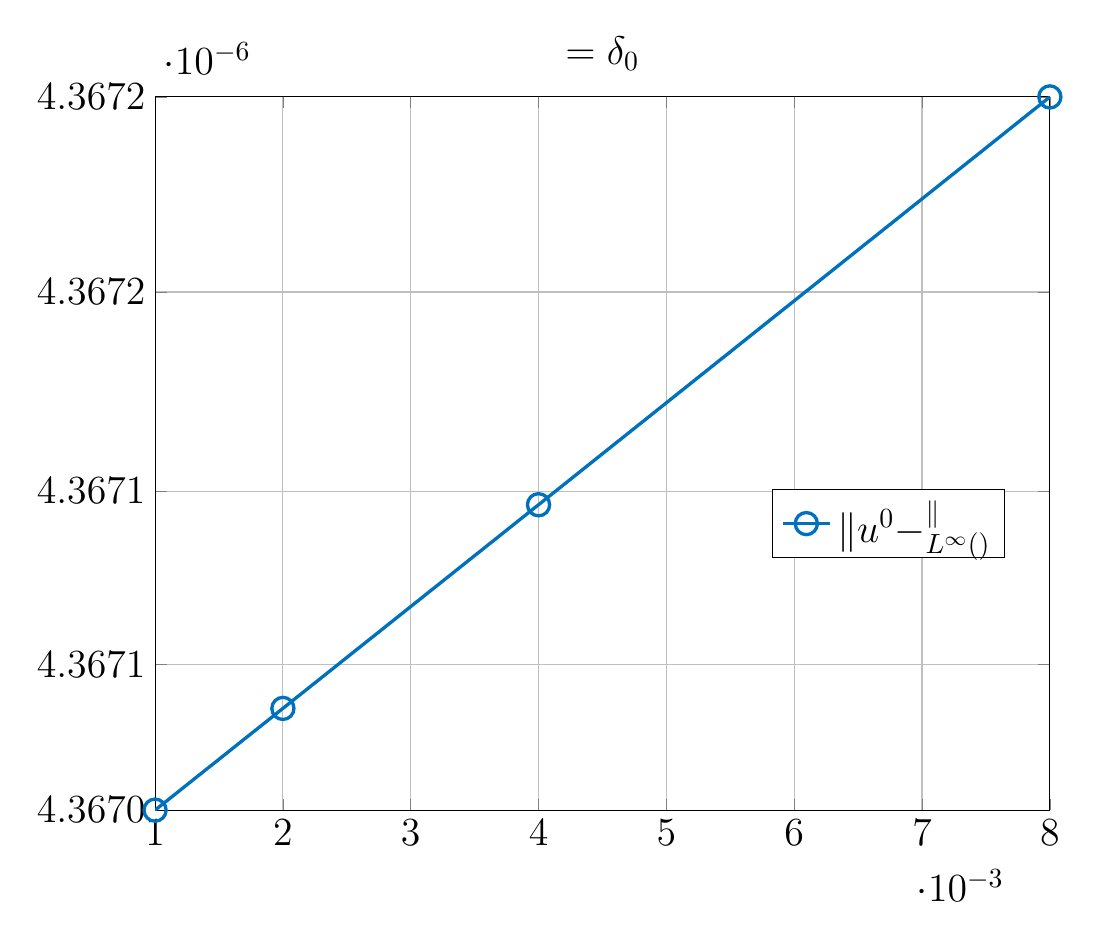
\begin{tikzpicture}[font=\Large]

\begin{axis}[%
compat=newest,
width=4.474in,
height=3.566in,
at={(0.806in,0.481in)},
scale only axis,
xmin=0.001,
xmax=0.008,
xlabel style={font=\color{white!15!black}},
xlabel={\Large $\boldsymbol{\eps}$},
ymin=4.36704256742396e-06,
ymax=4.36721917009211e-06,
ytick={4.36704256742396e-06, 4.36707866742396e-06, 4.3671215742396e-06, 4.36717086742396e-06,	 4.36721917009211e-06},
ylabel style={font=\color{white!15!black}},
%ylabel={\Large $\|u^0-\uh^\eps\|_{L^\infty(\Ltwo)}$},
axis background/.style={fill=white},
title style={font=\bfseries},
xmajorgrids,
ymajorgrids,
yticklabel=\pgfmathprintnumber{\tick},
y tick label style={
	/pgf/number format/.cd,
	fixed,
	fixed zerofill,
	precision=4,
	/tikz/.cd
},
title={\Large $\frakK=\delta_0$},
legend style={at={(0.95,0.45)}}
]
\addplot [color=mycolor1, mark=o, mark size=4pt, mark options={solid, mycolor1},  line width=1.2pt]
table[row sep=crcr]{%
0.001	4.36704256742396e-06\\
0.002	4.36706775770083e-06\\
0.004	4.36711818709765e-06\\
0.008	4.36721917009211e-06\\
};

\addlegendentry{$\|u^0-\uh^\eps\|_{L^\infty(\Ltwo)}$}
\end{axis}


\end{tikzpicture}%
\end{adjustbox}	% This file was created by matlab2tikz.
%
\definecolor{mycolor1}{rgb}{0.00000,0.44700,0.74100}%
%
\begin{adjustbox}{width=0.45\linewidth}
\begin{tikzpicture}[font=\huge]

\begin{axis}[%
compat=newest,
width=6.028in,
height=4.754in,
at={(1.011in,0.642in)},
scale only axis,
xmin=0.001,
xmax=0.008,
xlabel style={font=\color{white!15!black}},
xlabel={\huge $\boldsymbol{\eps}$},
xtick={0, 0.002, 0.003, 0.004, 0.005, 0.006, 0.007, 0.008},
ymin=4.36705490084247e-06,
ymax=4.36731790400859e-06,
ytick={4.36705490084247e-06, 4.36711365084247e-06, 4.36717684084247e-06,  4.36725240084247e-06, 4.36731790400859e-06},
format/.cd,
ylabel style={font=\color{white!15!black}},
%ylabel={\huge $\|u^0-\uh^\eps\|_{L^\infty(\Ltwo)}$},
axis background/.style={fill=white},
title style={font=\bfseries},
title={\huge $\frakK= \dfrac{1}{\Gamma(1-\alpha)}t^{-\alpha}$,\quad ${\alpha=0.6}$},
xmajorgrids,
ymajorgrids,
yticklabel=\pgfmathprintnumber{\tick},
    y tick label style={
	/pgf/number format/.cd,
	fixed,
	fixed zerofill,
	precision=4,
	/tikz/.cd
},
%legend style={legend cell align=left, align=left, draw=white!15!black}
legend style={at={(0.95,0.45)}}
]
\addplot [color=mycolor1, mark=o, mark size=5.1pt, mark options={solid, mycolor1},  line width=1.2pt]
  table[row sep=crcr]{%
0.001	4.36705490084247e-06\\
0.002	4.36709244792076e-06\\
0.004	4.36716755458297e-06\\
0.008	4.36731790400859e-06\\
};
\addlegendentry{$\|u^0-\uh^\eps\|_{L^\infty(\Ltwo)}$}
\end{axis}

\end{tikzpicture}%
\end{adjustbox}
	\caption{Convergence of solutions of \eqref{Ph_nl} for fixed $h$ as $\eps \rightarrow 0$}
	\label{Fig:epsConv1D}
\end{figure}
~\\

\indent In case of the time-fractional evolution, we follow the approach of~\cite{kaltenbacher2022fractional} and combine the Newmark method with an $L^1$-type scheme for the fractional derivative. The latter relies on the following approximation of the derivative of order $\alpha$ of $\uh^\eps$ at the time step $t_n$:
\begin{equation}
\begin{aligned}
\textup{D}_t^\alpha \uh^\eps(t_n) =&\, \frac{1}{\Gamma(1-\alpha)} \sum_{j=0}^{n-1}\int_{t_j}^{t_{j+1}} (t_n-s)^{-\alpha}\uht^\eps(s) \ds \\
\approx&\, \frac{1}{\Gamma(1-\alpha)} \sum_{j=0}^{n-1}\frac{\uht^\eps(t_{j+1})+\uht^\eps(t_j)}{2}\int_{t_j}^{t_{j+1}} (t_n-s)^{-\alpha} \ds \\
=&\, \frac{1}{2\Gamma(2-\alpha)} \sum_{j=0}^{n-1}\left(\uht^\eps(t_{j+1})+\uht^\eps(t_j)\right)\left((t_n-t_j)^{1-\alpha}-(t_n-t_{j+1})^{1-\alpha}\right);
\end{aligned}
\end{equation}
we refer to~\cite[Sec.\ 2.1]{kaltenbacher2022fractional} and~\cite{jin2019numerical} for details. The nonlinearity is resolved through a fixed-point iteration with the tolerance set to $10^{-8}$. The final time is set to $T=0.25$. We conduct a sequence of simulations of \eqref{Ph_nl} where we set
\begin{equation}
\begin{aligned}
\eps \in \{1, 2, 4, 8\} \times 10^{-3}.
\end{aligned}
\end{equation}
The spatial discretization parameter and time step are fixed beforehand so that $h^2$, $\Delta t << 10^{-3}$. The error $\|u-\uh^\eps\|_{L^\infty(\Ltwo)}$, plotted in Figure~\ref{Fig:epsConv1D}, is of order one, as expected for the semi-discrete solution, indicating the same behavior for the fully discrete method in the present setting.
\section*{Conclusion}
In this work, we have determined sufficient conditions under which finite element discretizations of Westervelt-type equations with strong or time-nonlocal damping preserve the vanishing dissipation asymptotics. We have furthermore established the rate of convergence with respect to the perturbation parameter $\eps$. Future work will be concerned with the analysis of time discretization schemes in the asymptotic-preserving regime.
\section*{Acknowledgments}  The author is thankful to Mostafa Meliani (Radboud University) for the careful reading of the manuscript and helpful comments.